\section{CrashSimulator Approach Details}
    %%% This figure is definitely wrong. Will recreate %%%
    \begin{figure}[t]
        \center{}
        \fbox{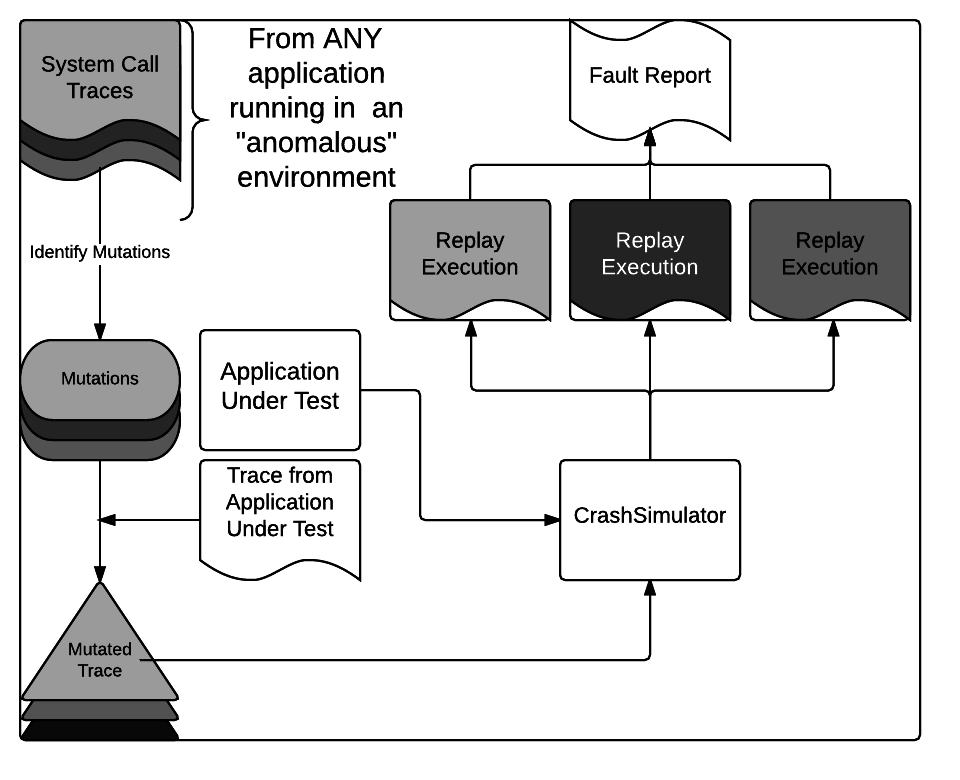
\includegraphics[scale=.5]{Architecture}}
        \caption{High level view of CrashSimulator's Architecture.}
        \label{figure:architecture}
    \end{figure}

    \subsection{CrashSimulator's Approach}
    
    CrashSimulator's testing process is based on two concepts: evaluating an
    applications behavior based on the system calls it makes in a given
    situation and the deterministic replay of a system call trace recorded from
    the application being tested.  Prior to beginning CrashSimulator's testing
    process, a set of bad behaviors (which we refer to as anomalies) to test for
    must be identified.  This can be accomplished either manually or by
    examining applications running in the target environment with existing
    tools.  This work utilized the results of both NetCheck and CheckAPI, as
    well as manual analysis, to develop the set of anomalies used in our
    evaluation.  NetCheck readily able to identify a wide variety of anomalous
    behaviors related to network communication between one or more
    hosts. CheckAPI peforms a similar function by comparing ``behavior of an API
    implementation to a reference model.''

    Another source of anomalies is the public bug trackers of projects available
    on the web.  The presence of a bug can be defined as a series of system
    calls then a model that identifies during execution can be constructed. This
    is ideal when determining whether or not an application is vulnerable to a
    widely publicized bug.  Similarly, bugs can be taken from similar projects
    in order to expand a project's ``test suite.''

    Once an anomaly has been identified, it is distilled into the sequence of
    system calls that ``implement'' the anomalous behavior.  This process
    involves examining the traces containing anomalies in order to identify a
    series of system calls indicative of the presence of the anomaly.  This
    analysis should identify two things: what mutations, if any, need to be made
    to a to the to-be-replayed system call trace to simulate the anomalous
    environment and what system calls the application should make in order for
    the replay execution to be accepted.

    CrashSimulator can use the outputs of this analysis either as mutations to
    be applied to a system call trace of the application under test or as input
    to a ``checker'' that determines whether an application has performed a
    required set of actions. When a ``checker'' is required, the sequence of
    system calls is encoded as a computational model that, when provided with as
    input the system calls made during the course of an execution, can decide
    whether or the series of system calls is present.  If the analysis reveals
    that anomalous conditions need to be injected into a replay execution this
    is facilitated by modifying the to-be-replayed system call trace from the
    application under test.

    In some cases, only one of these pieces is required for CrashSimulator to
    perform its analysis.  If there is not a definite correct response system
    call sequence, CrashSimulator's default checker can be employed to determine
    whether the application has noticed the anomaly and whether it may be making
    an effort to handle it.  As an example of this situation refer to the our
    evaluation section on ``unusual file type bugs.''  From the other direction,
    CrashSimulator can employ more specific checkers in a replay execution of an
    application performing some task in order to determine whether it handled
    all the edge cases it should have.  We employed this technique in our
    evaluation of CrashSimulator in finding bugs related to moving files across
    devices.

    %Consider the example of an anomaly identified in a web server application.
    %This behavior can distilled down to a series of system calls indicitive of
    %the anomaly.  If this behavior is present in other network-reliant
    %applications it too can be identified by looking for the same series of
    %system calls.  This series of system calls can then be transformed into a
    %computational model as described above.  As another example, consider the
    %bugs in Python's shutils that were discussed earlier.  In the case of the
    %``race condition'' bug, the series of system calls indicative of its
    %presence is an application using stat() to check a file, open() to open it,
    %and a series of read() and write() calls to copy its contents to the
    %destination without a call to fstat() that to confirm that the file was not
    %modified after the initial call to stat().

    The next step in CrashSimulator's testing process is to run CrashSimulator's
    replay tool against the application being tested.  The replay process
    consists of CrashSimulator launching the application under test as a child
    process and interceeding in its execution at approprate times in order to
    simulate the results and side effects of any system calls the application
    makes.  Because the system call trace being replayed has been mutated to
    reflect the chosen anomalies, exposes the applications to those
    anomalies. After the replayed execution concludes, CrashSimulator able to
    use the ending state of its checkers to report whether or not anomalous
    behavior was present.  The up front effort in this process only needs to be
    done once. One of CrashSimulator's major advantges over application-specific
    test suites is that checkers and, if necessary, any associated system call
    trace mutations can be accumulated and used to test any application
    CrashSimulator's user is interested in.

    %In the case of the Python
    %shutils race condition, the faulty behavior can be identified using a simple
    %python script that calls shutils.move() to move a file between directories
    %located on different storage devices.  CrashSimulator is able to identify
    %the bad behavior by replaying a system call trace taken of an execution of
    %the Python interpreter while it executes the script in question.

    %For example, a set of bugs that will be
    %discussed later were found by modifying a rename() system call to return a
    %result indicating that the application is attempting to move a file across
    %disks -- an operation the system call cannot perform.  In a well behaved
    %application, this will trigger an alternative execution path wherein the
    %file is manually copied by the application.  In a buggy application either
    %this case will be handled incorrectly (i.e. the appliation will fail to
    %perform all of the steps required to properly copy a file across devices, a
    %situation caught by well-constructed anomaly models) or will not be handled
    %at all, that is, the application will fail eventually because it did not
    %recognize that the call to rename was not successful.

    %I feel like this is important to include but am having trouble figuring out
    %where to put it.
    
    \paragraph{The Default Checker}

    When CrashSimulator injects anomalous behavior into a replay execution it is
    done with the intention that the application under test deal with this
    anomaly in some way. For example, if CrashSimulator modifies the data
    structure returned by a call to {\tt stat64()} such that the target file
    appears to be a symlink rather than a regular file, the application should
    take some action to deal with this fact.  There are numerous ways an
    application could correctly handle a given anomaly so CrashSimulator must
    generically accept all of them.  The ``default checker'' handles this by
    making the assumption that an applications efforts to deal with the anomaly
    will result in it executing different program paths (and threfore different
    system calls) than were executed when the system call trace being replayed
    was recorded.  Based on this, if the application being replayed does not
    alter its behavior to deal with this the anomaly, the application has not
    correctly handled the anomaly -- a failing result.  Alternatively, if the
    application deivates from the behavior recorded in the system call trace
    driving the replay it is likely that the application is taking some action
    to handle the injected condition -- an indiciation of possibly correct
    behavior.

    This approach is sufficient because in reality, a test can only tell us if
    an application performs a specific bad behavior in a specific situation.  A
    test cannot prove that an application is bug free in the same situation.  As
    with traditional tests, CrashSimulator cannot tell us that an applcation is
    bug free in a given situation -- instead it can assert that an application
    has incorrectly handled a given situation based.
    

    \paragraph{More Specific Checkers}

    CrashSimulator also accepts more specific checkers that evaluate wether or
    not an application has performed a required operation.  These checkers
    monitor a replay execution for a specific system call sequence (with the
    correct parameters, return values, and state modifications) that indicates
    the application has carried out the operation in question.  To achieve this
    these checkers contain a computational model (e.g. a deterministic finite
    automaton, a push down automaton, etc.) that encodes and accepts the
    system call sequence it has been constructed to watch for.  Whether
    CrashSimulator ultimately accepts a given replay execution is determined by
    the ending states of the checkers monitoring the execution.


    \subsection{Architecture}
        
    At a high level CrashSimulator is organized into two primary modules. The
    first module is responsible for monitoring a given execution, determining
    when to inject anomalous behavior, and determining whether or not the
    application responded correctly to the injected behavior. The second module
    is responsible for managing the execution of the application under test such
    that it precisely follows a previously recorded system call trace -- a
    process we refer to as ``replaying'' a system call trace.

    %The first step in CrashSimulator's work flow is to identify anomalous behavior in an arbitrary application.
    %Currently, this step is accomplished through manual bug hunting and through examination of diagnostic output from
    %NetCheck and CheckAPI. CrashSimulator's user examines the system call behavior that resulted in this bad behavior
    %and constructs a model that defines what triggers the anomalous behavior and the subsequent ``bad'' system call
    %behavior (\emph{Do we need to say something about future work doing this step automatically here?}.
    %CrashSimulator's first module operates by using this model to analyzed the system call behavior of the application
    %under test(e.g. order, parameters, side effects, return values).
        
    CrashSimulator's makes use of the Ptrace facilities built into modern
    versions of the Linux kernel. The aforementioned ``replay'' of a system call
    trace is achieved by intercepting every system call the application makes,
    preventing the actual system call from being carried out by the kernel
    (i.e. no-oping out the real system call by replacing it with a call to
    getpid()), identifying the matching system call from the previously recorded
    trace, and replicating the return value and side effects such that the
    application believes that the system call it made actually took place. We
    have found that emulating the post conditions of the system calls an
    application makes results in faithful replay of a previous execution in most
    cases.


    CrashSimulator is fully self contained and operates without user
    intervention during its analysis process. At this point, CrashSimulator
    itself is available as a virtual machine appliance compatible with the
    \emph{Virtual Box} virtual machine hosting software.  The reasons for
    distributing CrashSimulator in this manner are threefold.  First, this
    distribution method ensures that all of CrashSimulator's dependences are
    installed and configured appropriately.  Second, this method provides an
    environment for taking system call traces that is known to be complete
    tool-wise and compatible with CrashSimulator.  Finally, and most importantly,
    this method provides an environment that is known to be compatible with the
    details of CrashSimulator's system call replay techniques.

    CrashSimulator's source code is available and, while other environments may
    be untested, it should function correctly on any platforms that meet the
    criteria described above.

    \subsection{System Call Traces and Replay}

        \subsubsection{Why System Call Traces?}

        In order to inject anomalies and monitor program behavior as described
        above, CrashSimulator needs to have detailed interactions with the
        application under test at some level.  The option of carrying out these
        interactions at the system call level was chosen because for several
        reasons:

        \paragraph{Tooling}

        Operating at the system call level allows this work to take advantage of
        two key pieces of tooling that already exist in mature form on Linux.
        The first is ptrace. {\tt Ptrace} is a process manipulation interface provided
        by the Linux kernel whose primary use case is debugger development.
        This work leverages {\tt ptrace} in order to start and stop execution of a
        process as well as read and write the contents of the processes
        registers and memory.  Using these operations allows CrashSimulator to
        pause execution before and after each system call an application makes
        in order to manage execution and inject anomalies where appropriate.

        This CrashSimulator also relies on system call traces recorded using
        strace.  The strace system call trace format is extensive and captures
        the parameters, return values, and side effects of each system call an
        application makes.  Such a record provides CrashSimulator with all the
        information needed to direct execution of the application in such a way
        that the contents of the system call trace are faithfully replayed.  It
        is in this way that system call traces act as an interface over an
        applications execution that used to inject anomalous behavior.

        \paragraph{Removal of language dependence}

        Operating at the system call level means that CrashSimulator is not
        dependant on a particular programming language or runtime.  This means
        that CrashSimulator does not require any complext language parsing and
        analysis code while still allowing it to posess many of the benefits of
        systems that perform such work.  Tools that perform language parsing do
        so in order to craft inputs that specifically exercise target execution
        paths in an application.  This work is concerned with issues that arise
        at the ``interfaces'' between an application and its environment.
        Manipulating system calls allows us to skip the process of generating
        these crafted inputs to this end in favor of directly effecting the
        behavior we are interested in.

        \paragraph{Identify Issues that Result from an Application's Environment}

        Most current testing strategies are very application-centric.  For
        example, a black box fuzzer is able to identify faults that arise when
        an application begins processing data it has received from a network
        connection. CrashSimulator, on the other hand, is able to identify
        issues that arisese from the network connection itself.

    \subsubsection{Why Replay Executions?}

        Replay is important because it allows CrashSimulator to execute an
        application free from dependencies on things like file system contents,
        network configuration, or communication with other applications.  For
        example, if an application depends on a file being present in a filesystem,
        CrashSimulator can intercept calls to {\tt read()} from and {\tt write()} to
        this file removing the need for this file to actually be present during
        replay executions. Additionally, replay allows CrashSimulator to reproduce
        the differences between version of libraries and other executable
        dependencies alleviating the need install them in the test environment.

    %\paragraph{Control Execution}

    %Because it is simulating aspects the application under test's environment, CrashSimulator is able to manipulate the
    %data the application receives from these aspects in order to control execution.  This is the key feature that allows
    %CrashSimulator to inject anomalous situations into an execution.  For example, by simulating the communications
    %between the application under test and another host on a network, CrashSimulator can fragment, modify, or even drop
    %data ``incoming'' from the simulated remote host in order to determine whether or not the application appropriately
    %handles the situation. 